% LOrkCraft Paper for NIME 2013 
%
% Using the LaTeX Template for NIME 2013

\documentclass{nime-document-class}

\begin{document}

\conferenceinfo{NIME'13,}{May 27 -- 30, 2013, KAIST, Daejeon, Korea.}

% use \projectName{} to refer to the project in the paper
% makes changing it later much easier - just change it here!
\newcommand{\projectName}{LOrkCraft}

\title{\projectName{}: Making Music While Playing Starcraft 2}

\numberofauthors{3}
\author{
% 1st. author
\alignauthor
Mark Cerqueira\\
       \affaddr{Smule, Inc.}\\
       \affaddr{577 College Avenue}\\
       \affaddr{Palo Alto, California}\\
       \email{mark@smule.com}
% 2nd. author
\alignauthor
Spencer Salazar\\
       \affaddr{Center for Computer Research in Music and Acoustics (CCRMA)}\\
       \affaddr{Stanford University}\\
       \email{spencer@ccrma.stanford.edu}
% 3rd. author
\alignauthor
Ge Wang\\
       \affaddr{Center for Computer Research in Music and Acoustics (CCRMA)}\\
       \affaddr{Stanford University}\\
       \email{ge.stanford.edu}
}

\maketitle
\begin{abstract}
\projectName{} is a framework that enables real-time data gathering from a {\em Starcraft 2} match to external audio servers via Open Sound Control allowing a match played between individuals to become a live performance piece.
While players battle each other for victory as they normally do, a custom {\em Starcraft 2} map collects and writes out data about player's decision-making, performance, and current focus on the map.
This data is parsed and transmitted over OSC in real-time and becomes the source for the sonic piece that accompanies the player's game.
This paper details the technical and aesthetic decisions made during the development of \projectName{}, covering data collected during the game and discussing the sonic mappings explored.
\end{abstract}

\keywords{NIME, Starcraft 2, sonification, music}

\section{Introduction}
{\bf Introduce the premise behind using data from a video game to make music.}

\section{Background}
\projectName{} centers around the widely popular RTS or "real-time strategy" video game series {\em StarCraft 2} by Blizzard Entertainment ~\cite{Blizzard:2013:Online}.
In {\em StarCraft 2}, players can control one of three distinct races: the Terrans, humans who were exiled from Earth long ago; the Zerg, an insectoid alien species obsessed with overrunning assimilating other species; and the Protoss, a humandoid species with advanced technology and great psionic abilities seeking the annihilation of the Zerg ~\cite{BlizzardRaces:2013:Online}.
While the game features a story-driven campaign mode, most StarCraft players spend their time on the ladder, battling out against other players over the internet. 

During a match, players see the action from a top-down perspective and only have vision of the map where they have units or buildings present.
Players switch between building up their economy by constructing workers that collect resources or building an army to attempt to do damage to their enemy.
A player who is able to build a strong economy and the proper number and composition of units that counter their opponent's units will be in an advantageous position.
The game ends when a player destroys the other player's structures or the other player surrenders.

\section{Related Work}
\projectName{}'s use of a video game as an interface for producing music is directly influenced by many other works in the computer-music community.

In the 2008 paper, {\em Composing for Laptop Orchestras}, founding members of the Princeton Laptop Orchestra, PLOrk, discuss the possibilities of using games in computer music environments and some of the game pieces they developed.
One early and relevant piece to \projectName{} is Scott Smallwood's {\em The Future of Fun (1983)!}, which has each performer playing a different game from the Multiple Arcade Machine Emulator (MAME).
Performers pick a game from MAME, which features games from the early 1980s arcade-game era, such as {\em Pac-Man}, {\em Defender}, and {\em Donkey Kong}, and they play the game for a specified amount of time.
The sounds each game produce become the piece and while different from game to game, produce a soundscape of low-resolution synthetic sounds common to the times ~\cite{ComposingForLaptopOrchestra:Article}.

% if there are not more relevant examples
\iffalse
The first such piece discussed is Scott Smallwood's {\em On the Floor}, which presents performers with a slot machine interface and thirty credits.
Performers can bet between one and three credits each time on the slots and normal slot-machine sounds are generated.
A conductor monitors win rates and tweaks win chances to ensure everyone is eventually a loser.
As the performers lose credits and cross a credit threshold, looped recordings from an actual casino begin to play.
Inevitably, once the user runs out of credits each performer is left with a drone and the piece concludes once all performers have run out of credits. 
\fi

\section{System Overview}
\projectName{} consists of a set of utilities that work in tandem to get data from a live StarCraft 2 match to OSC clients that sonify the game.
The main components include a custom Starcraft 2 map, a Ruby parser and OSC dispatcher, and our audio engine.

\subsection{Creating the Custom Map}
An existing Starcraft 2 map, Antiga Shipyard created by Blizzard shown in (Figure~\ref{fig:AntigaShipyardFigure}), was modified to collect various data in real-time during a game.
These {\em triggers} fire off either periodically (every 2 seconds) or after certain events (a unit is produced). When a trigger fires, data is collected and written to XML bank files.
The map created for \projectName{} is for two players, but the triggers can be shared to any other map with any number of players. 

\begin{figure}[htbp]
	\centering
		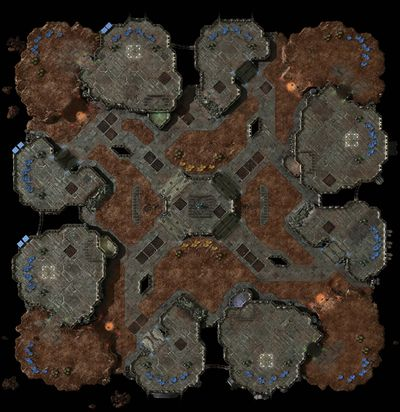
\includegraphics[width=1\columnwidth]{antiga-shipyard}
	\caption{The Antiga Shipyard map. Players start in the bottom right or top left positions.}
	\label{fig:AntigaShipyardFigure}
\end{figure}

Data collected during the game focuses on player actions and current state of the player's army.
Tracked data includes:
\begin{itemize} \itemsep1pt \parskip0pt \parsep0pt
  \item Coordinates where a player is currently focused on the map
  \item Composition of the player's standing army
  \item Units being produced by the player and their current build progress
  \item The player's effective actions per minute (APM)
  \item Various metrics about a player's economic health including mineral and vespene gas collection rate as well as harvesters built and lost
  \item Total number of enemy units destroyed and structures razed
  \item The player's general {/em score} that combines all these factors to produce a single number that is normally a good indicator of performance (this is typically only shown after a match has ended) \ldots
\end{itemize}

\subsection{Parsing and Sending Game Data}
A Ruby script monitors the directories that contain these bank files using guard/listen and when the files are updated, the data is parsed out of the XML bank files using Nokogiri and that data is sent to any listening OSC clients that handle sonification or visualization.
Unfortunately, this is the only {\em legitimate} way to get data out of Starcraft 2, but we found the latency between a trigger being fired and an OSC client receiving the message to be acceptable given we had fine control over how often our script polls the file system for bank file updates.
With OS-specific file system polling adapters, the overhead of writing to a file and parsing the data out of that file became negligible in tests.

\subsection{Sonification of Game Data}
{\bf What we did with the OSC messages.}

\subsection{Conclusion}
{\bf What we want people to do with \projectName{}.}

% Acknowledgments are optional
\section{Acknowledgments}
We would like to thank Tasteless and Artosis for being awesome.

\bibliography{nime-references}{}
\bibliographystyle{abbrv}

% Place this command where you want to balance the columns on the last page. 
% \balancecolumns 

\end{document}
